\section{THC, Was ist das?}
\rhead{THC, Was ist das?}

Die "THC", ausgeschrieben thermohaline Zirkulation. Ist eine Weltumspannende Meeresströmung welche in verschiedene Abschnitte aufgeteilt werden kann.
Diese Strömungen sorgen für eine Durchmischung der verschiedenen Ozeane. So erzeugen sie einen Wärme- und Nährstoffaustausch in den verschiedenen Weltregionen. 
Die Auswirkung dieses Energieaustausches sind spürbar, so heizt zum Beispiel der Golfstrom, welcher Auch zu diesen Strömungen gehört Nordeuropa um mehrere Grad auf.
Doch wie entsteht diese Strömung?
Hier spielen viele Einflüsse eine Rolle. Die Verteilung der Kontinente, die Corioliskraft, die Wasserdichte und auch Wetter und Winde. 
Im Rahmen dieser Arbeit werde ich nur auf die Wasserdichte als Einfluss eingehen. Sie ist gut zu simulieren und ist durch die einfache Veränderbarkeit auch am Spannendsten.
die Verteilung der Kontinente und auch die Corioliskraft sind durch ihre kaum vorhandene Änderung als Konstanten zu betrachten. Das Letzte was noch bleibt, sind Wind und Wetter. 
Diese Einflüsse sind praktisch nicht vorherzusagen und auch ihr Einfluss variiert stark. Aus diesem Grund werden auch diese nicht Simuliert. 
Zusätzlich würde das Einbeziehen dieser grössen die Komplexität der Simulation Stark erhöhen.

\subsection{Dichte}
\rhead{Dichte}

Die Thermohaline Zirkulaton wird hauptsächlich durch Dichteunterschiede im Wasser hervorgerufen.
Dichtes Wasser sinkt ab und weniger dichtes Wasser steigt bekanntlich auf. Die Hauptsächlichen Einflussfaktoren der Wasserdichte sind:

\begin{itemize}
	\item Salzgehalt
	\item Temperatur
\end{itemize}

Durch einen hohen Salzgehalt wird das Wasser dichter. Die Temperatur hat den inversen Einfluss. Je wärmer das Wasser wird, desto weniger dicht ist es. 
Hier zwei Grafiken zur Veranschaulichung:
\begin{figure}
\includegraphics{code/graphs/graph_salinity.jpg}
\caption{Dichteveränderung abhängig vom Salzgehalt}
\end{figure}

\begin{figure}
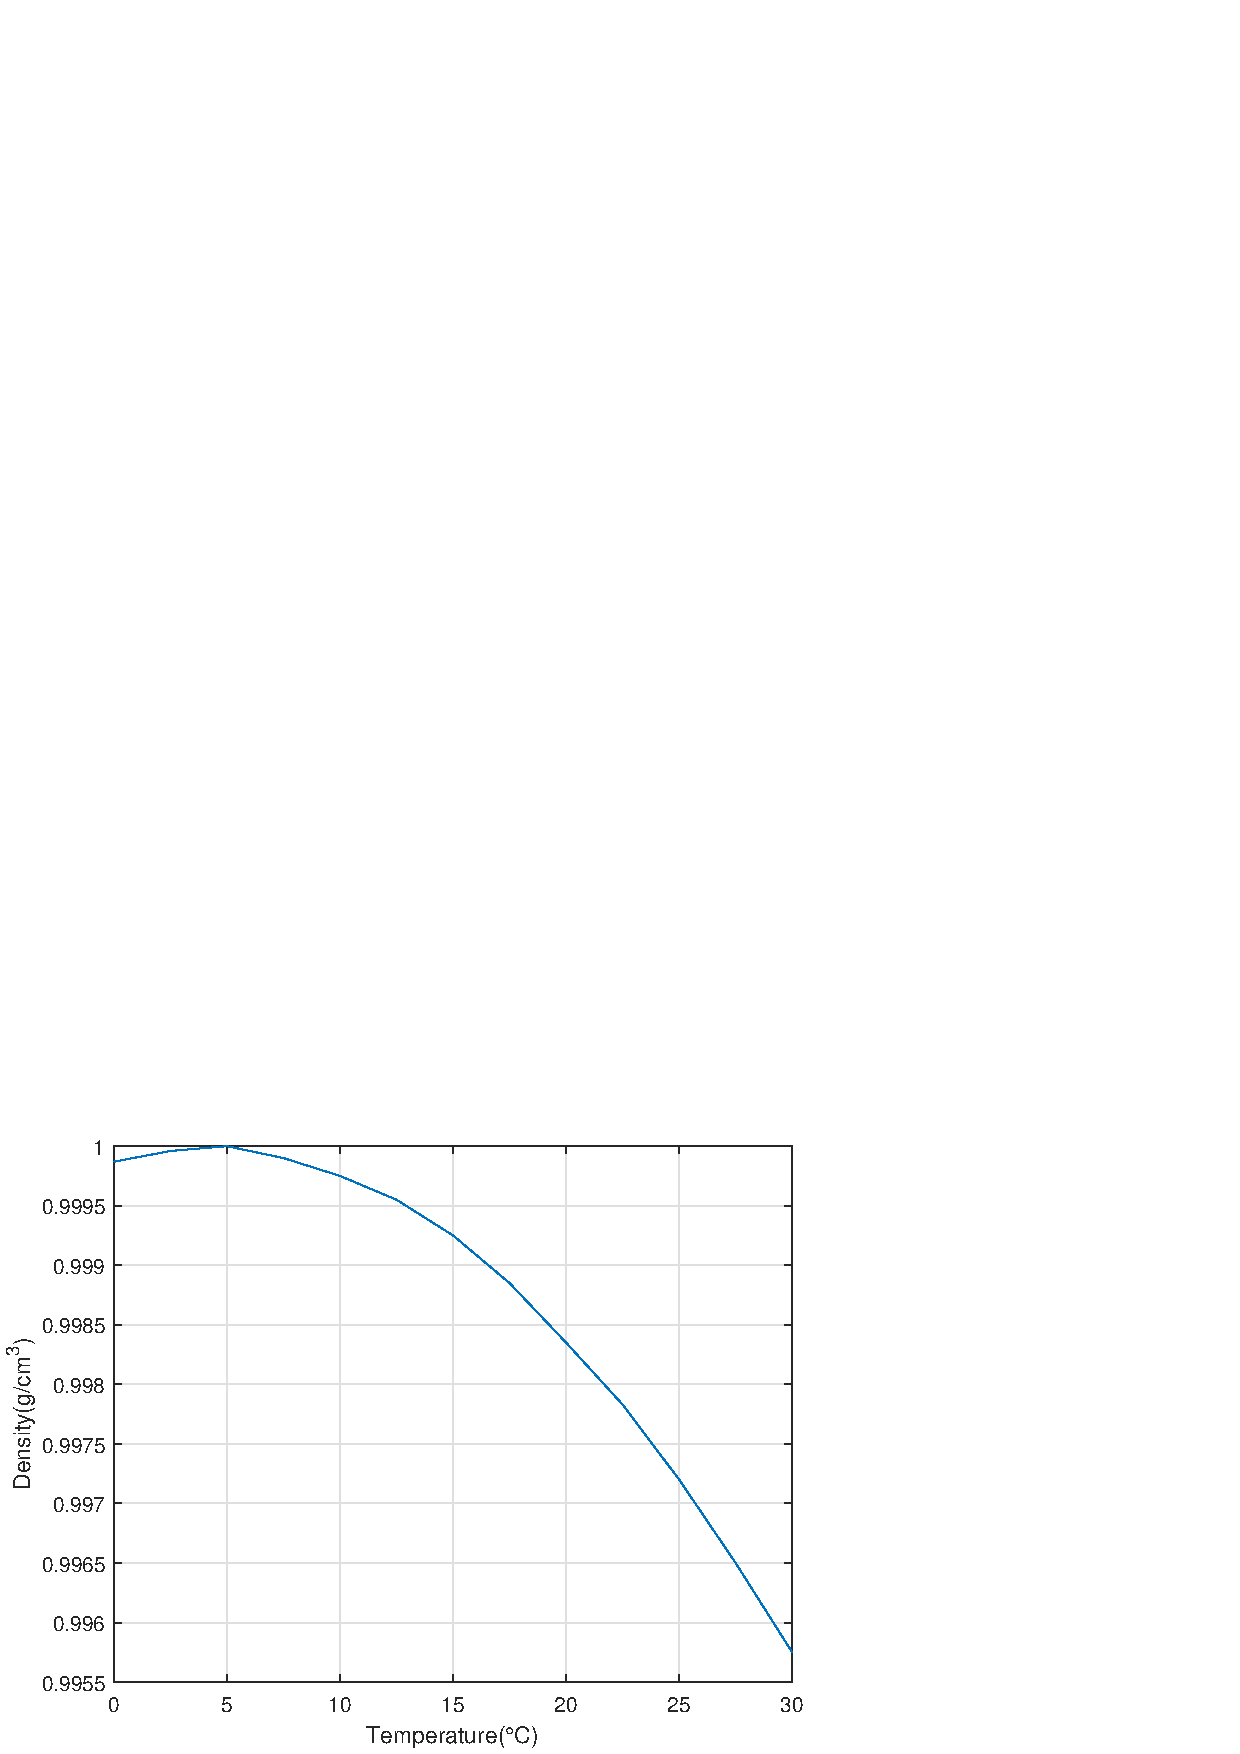
\includegraphics{code/graphs/graph_temp.jpg}
\caption{Dichteveränderung abhängig von der Temperatur}
\end{figure}

Diese Einflüsse Lassen sich in einer Gleichung zusammenfassen, welche im Hauptteil des Buches im Kapitel \ref{Salinität und Dichte} schon Besprochen wurde.

\begin{equation}
\varrho
=
\varrho_0(1-\alpha(T-T_0)+\beta(S-S_0))
\label{skript:salinity-linear}
\end{equation} 

Mittels dieser Gleichung lässt sich nun ein Simulation erstellen, mit welcher sich solche Strömungen simulieren lassen.

\subsection{Golfstrom}
\rhead{Golfstrom}

Im Rahmen dieser Arbeit habe ich versucht den Golfstrom, welcher Europa direkt beeinflusst, zu Simulieren.
Als fokussieren ich hier nur auf einen kleinen Teil der Globalen Thermohalinen Zirkulation.


\begin{figure}
	\includegraphics[]{bilder/deep_ocean_currents.jpg}
\end{figure}

Die Frage ist nun, was passiert mit dem Golfstrom, wenn Klimaerwärmung und Umweltverschmutzung weiter ansteigen?

\subsubsection{Funktionsweise}

Doch zuerst dazu, wie der Golfstrom funktioniert.
Der Golfstrom entspringt im Golf von Mexiko. Von dort aus wird das Warme Wasser von Winden und der Erdrotation nach Norden getrieben.
Auf diesem Weg kühlt das Wasser langsam ab, und wird durch die fortlaufende Verdunstung von Wasser immer salziger. Da der Einfluss der Salinität grösser ist als der der Temperatur, beginnt das Wasser im Norden, durch die nun Hohe Dichte abzusinken. Wenn das Wasser dann abgesunken ist, treibt es dem Grund des Meeres entlang bis nach Afrika, was den Kreislauf schliesst.
Wo hat der Klimawandel nun seinen Einfluss?
Um diese Frage zu beantworten, müssen wir weiter zurückschauen, genauer gesagt zum Kap der guten Hoffnungen. Denn eigentlich beginnt die Strömung schon dort. 
Dort Stellt sich die Frage, in welcher Richtung der Indische Ozean und der Atlantik ihr Salz austauschen. 
Denn eine Veränderung der Salzbilanz könnte im Norden, also vor der Küste Grönlands für eine Störung des Absinkens sorgen, und so den Strom zum erliegen bringen. 
Eine Störung der Salzzufuhr könnte also den Golfstrom zum erliegen bringen.
Hier gehen die Meinungen der Forscher jedoch auseinander. Salzmessungen im offenen Meer sind sehr schwierig. 
Im Moment zeigen diese jedoch, dass der Golfstrom weiter Salz in den Atlantik importiert und sich so selber am leben erhält.

Weiter kommt da noch die Erhöhung des CO2-Gehaltes in der Luft und die somit einhergehende Klimaerwärmung. sie hat zwei direkte Auswirkungen auf den Golfstrom:

\begin{itemize}
	\item Durch die Erhöhung der Lufttemperatur kann das Wasser auf dem Weg in den Norden nicht mehr genug abkühlen, um danach abzusinken.
	\item Das Abschmelzen der Polkappen, welches viel Frischwasser freisetzt, kann die Salzkonzentration so weit verringern, dass das Wasser, aufgrund der reduzierten Dichte, nicht mehr absinken kann.
\end{itemize}

Diese Beiden Prozesse, wären alleine in der Lage den Golfstrom zu stören, doch zusammen ist die Wirkung noch viel schlimmer.

Laut einer Studie des Forschers Liu Wei von der Universität Yale vom 04 Jan 2017 könnte dieses Szenario in den nächsten 300 Jahren tatsächlich eintreten. Sie zeigen auf, dass falls sich die Rate seit 1990 verdoppelt, der Golfstrom in den nächsten 300 Jahren versiegen könnte.

\subsubsection{Folgen}

Was passiert, falls der Golfstrom zum erliegen kommt, oder sogar seine Richtung ändert.
Ich denke der Film "The day after tomorrow" von Roman Emmerich ist bekannt. Er zeigt was passieren könnte, falls der Golfstrom zum erliegen kommt. 
Im Film versinkt innert weniger Tage die ganze Welt in einer neuen Eiszeit un alles endet im Chaos. 
Das ist natürlich ein wenig übertrieben Dargestellt, doch die Richtung stimmt. Falls der Golfstrom stoppt, würde trotz Klimaerwärmung Nordeuropa um einige Grad kälter werden.













	
	
	
	
	
	
	
	
	
	
	
	
	
\end